% Manuscript prepared for Entropy (MDPI), Information Theory section.
% Compile inside the official MDPI LaTeX template.
% Before submission, verify the journal option against the current MDPI template
% and complete all author declarations in the submission system.
\documentclass[entropy,article,submit,pdftex,moreauthors]{Definitions/mdpi}

\Title{Information Leakage from Token-Length Traces in Streaming LLMs: Cross-Model Reconstruction and Defense Evaluation}
\Author{Paweł Augustynowicz $^{1,*}$ and Szymon Jędrzejczak $^{1,*}$}
\AuthorNames{Paweł Augustynowicz and Szymon Jędrzejczak}
\address[1]{Faculty of Cybernetics, Military University of Technology, gen. Sylwestra Kaliskiego 2, 00-908 Warsaw, Poland; pawel.augustynowicz@wat.edu.pl (P.A.); szymon.jedrzejczak@wat.edu.pl (S.J.)}
\corres{Correspondence: pawel.augustynowicz@wat.edu.pl (P.A.); szymon.jedrzejczak@wat.edu.pl (S.J.)}

\pubvolume{1}
\issuenum{1}
\articlenumber{0}
\pubyear{2026}
\copyrightyear{2026}
\datereceived{}
\daterevised{}
\dateaccepted{}
\datepublished{}

\usepackage{booktabs}
\usepackage{multirow}
\usepackage{graphicx}
\usepackage{array}
\usepackage{longtable}
\usepackage{tabularx}
\usepackage{threeparttable}
\usepackage{amsmath}
\usepackage{enumitem}
\usepackage{placeins}
\usepackage{tikz}
\usetikzlibrary{arrows.meta,positioning,shapes.geometric,fit}
\usepackage{pgfplots}
\pgfplotsset{compat=1.18}

\abstract{Streaming large language model (LLM) services reveal message-size metadata even when payloads are encrypted. We isolate the information carried by token lengths using an explicitly optimistic observation model: an instrumented service emits one Server-Sent Events (SSE) application event per token, and the attacker receives the ordered event lengths. The traces are therefore SSE-equivalent laboratory observations, not event boundaries extracted from TLS, HTTP/2, or QUIC traffic. A fixed T5-based reconstructor was tested on 300 aligned prompts for each of seven open-weight victim models (2100 samples) with a 512-token generation budget. Mean term-frequency cosine similarity $\phi$ ranged from 0.568 for Qwen2.5-1.5B-Instruct to 0.030 for TinyLlama-1.1B-Chat, and 17 of 21 paired model comparisons remained significant after Holm correction. Five models clustered at mean $\phi$ of 0.517--0.568 with $\mathrm{LR}@0.5$ of 59.7--76.3\%; TinyLlama and Phi-3.5-mini remained at the floor (0\%). These cosine scores overstate usable recovery: ROUGE-1 precision stayed near 0.23--0.31 for the high-$\phi$ cluster, and qualitative examples at $\phi>0.5$ can be topically wrong. EOS-complete fractions ranged from 0\% (Phi-3.5-mini) to 65.7\% (Llama-3.2-3B). In a 30-prompt control study for two models, replacing the true trace with a shuffled, constant, or cross-prompt sequence lowered mean $\phi$ by 0.046--0.196, showing that the ordered trace contributes to recovery while also exposing a sizeable language-prior baseline. Five framing transformations evaluated on the same two models reduced the frozen reconstructor's mean score by 35.0--90.3\%. No defended model--configuration pair produced a sample with $\phi>0.5$; with $n=30$, however, the Wilson 95\% upper bound remains 11.4\% for each zero-count condition. On 512-token traces of those two models, five decoder seeds and a prompt-disjoint empirical MAP inverse (22 cells, 3300 reconstructions) gave between-seed SDs of 0.003--0.018. The MAP inverse recovered most of the frozen drop for bucketing and batching and did not restore the inflated frozen score of \texttt{pad\_32}. The study measures transfer of one reconstructor under a length oracle. It does not quantify mutual information, prove intrinsic model vulnerability, or establish passive exploitability on encrypted production traffic.}

\keyword{large language models; information leakage; side-channel analysis; server-sent events; traffic analysis; token-length traces; text reconstruction; privacy}

\begin{document}

\section{Introduction}
Interactive LLM services stream partial responses to reduce perceived latency. One implementation uses Server-Sent Events (SSE), with generated text carried in application events such as \texttt{data: \textless token\textgreater\textbackslash n\textbackslash n}. Encryption hides the event contents but not necessarily the shape of the communication. If application-event boundaries or correlated record sizes are observable, a sequence of lengths can reveal properties of the underlying tokens.

This paper separates two questions that are often conflated. The first is whether an ordered token-length trace contains exploitable information about a response. The second is whether a passive observer can recover that trace from encrypted production traffic. We study only the first question. An instrumented service emits exactly one SSE-equivalent event per generated token and records the event length before transport-layer processing. This length-oracle abstraction removes HTTP/TLS segmentation, buffering, retransmission, and multiplexing from the experiment. It is deliberately favorable to the attacker and is not presented as an end-to-end network exploit.

We build on Weiss \emph{et al.}, who reconstructed streamed responses from token-length patterns with a T5-based inversion pipeline~\cite{weiss2024prompt}. Our experiment asks whether that fixed reconstructor transfers across open-weight victim models and how much of its score is attributable to the true length trace rather than its language prior. It also tests simple framing transformations without retraining the attacker.

The study addresses three research questions:
\begin{enumerate}[label=\textbf{RQ\arabic*:},leftmargin=3.8em]
    \item Does the true ordered length trace improve lexical reconstruction over shuffled, constant, and cross-prompt traces?
    \item How well does one fixed Weiss-style reconstructor transfer across seven victim models, and are the observed differences distinguishable under prompt pairing?
    \item How do bucketing, fixed-width units, batching, and randomized padding change reconstruction scores, protected-payload size, and frame count against a frozen attacker, and does a prompt-disjoint MAP inverse recover those scores?
\end{enumerate}

The contribution is an artifact-backed benchmark rather than a new transport-level attack. It provides: (i) a controlled length-oracle protocol and no-signal controls; (ii) a prompt-aligned, seven-model transfer evaluation with uncertainty intervals and multiplicity-corrected tests; (iii) a two-model pilot of five framing configurations with explicit cost accounting; and (iv) a five-seed, prompt-disjoint MAP-inverse evaluation of those configurations on 512-token traces. The code, prompts, per-sample outputs, analysis scripts, and a reproducibility manifest are available at \url{https://github.com/jackaugustyn/LLeakM}.

\section{Related Work}
Side-channel attacks infer sensitive information from indirect observables such as timing and message size. Classical timing attacks showed that implementation-level leakage can defeat cryptographic protection without recovering plaintext directly~\cite{kocher1996timing}. Encrypted network applications likewise leak through packet sizes and timing. Keystroke inference, web-application traffic analysis, and website fingerprinting demonstrate that encryption does not hide communication shape~\cite{song2001timing,chen2010sidechannel,cai2012touching,sirinam2018deep}.

Traffic-analysis defenses transform that shape through padding, morphing, batching, or cover traffic. Traffic morphing attempts to make one traffic class resemble another, while subsequent studies show that efficient countermeasures may retain exploitable structure or impose substantial overhead~\cite{wright2009morphing,dyer2012peekaboo}. These trade-offs motivate reporting residual leakage together with bandwidth and latency costs rather than treating padding as a binary protection.

For generative AI, Weiss \emph{et al.} introduced T5-based sequence-to-text inversion and reported accurate reconstruction for 27\% of responses and topic inference for 53\% in their evaluated setting~\cite{weiss2024prompt}. Li \emph{et al.} subsequently studied API outputs that merge several tokens into one observable unit and showed that aggregation does not remove the side channel~\cite{li2026length}. Whisper Leak instead infers prompt topics from packet-size and timing patterns in encrypted LLM traffic~\cite{whisperleak2025}. Those studies address stronger deployment-facing threat models. The present work narrows the observation layer to ask a different question: how a fixed reconstructor transfers across victim models once a token-granular length trace is available, and how simple transformations affect that same reconstructor.

The reconstruction pipeline uses T5-style text-to-text transformers~\cite{raffel2020exploring}. Evaluation combines a reference-normalized Levenshtein distance~\cite{levenshtein1966binary}, ROUGE precision~\cite{lin2004rouge}, and one fixed term-frequency cosine score $\phi$. These are lexical measures. They should not be read as semantic correctness or disclosure of a usable answer.

\section{Materials and Methods}
\subsection{Threat Model and Objective}
We evaluate an attacker that receives the ordered byte lengths of SSE-equivalent application-layer events generated by an instrumented LLM service. The attacker is assumed to observe only the lengths of streamed application events, without access to prompts, generated tokens, or internal model information. This is a length-oracle abstraction: unlike a fully passive network attacker, it does not need to infer application-event boundaries from TLS, HTTP/2, or QUIC traffic. The resulting measurements, therefore, characterize the information available once token-level lengths are observable. They do not address the separate problem of recovering those lengths from encrypted traffic in real-world deployments.

The primary objective is to determine how accurately assistant responses can be reconstructed from application-event lengths alone. The experiment therefore addresses three tasks: (i) capture per-token traces during live inference, (ii) reconstruct text from the resulting length sequences, and (iii) compare the reconstructions with the generated responses. Prompts are used to elicit the reference responses but are never supplied to the reconstructor. Figure~\ref{fig:threat_model} summarizes this observation boundary.

\subsection{Information-Theoretic Interpretation}
Let $R$ denote the generated response and let $X=(L_1,\ldots,L_T)$ denote its ordered token-length trace under the laboratory serialization. A defense maps $X$ to an observable trace $Z=g(X,N)$, where $N$ is independent randomness when the transformation is randomized. The attacker produces $\widehat{R}=A(Z,U)$, with $U$ representing decoder randomness. The resulting Markov chain is
\begin{equation}
R \longrightarrow X \longrightarrow Z \longrightarrow \widehat{R}.
\end{equation}
The data-processing inequality gives
\begin{equation}
I(R;\widehat{R}) \leq I(R;Z) \leq I(R;X).
\end{equation}
Reconstruction above no-signal controls is therefore evidence that the evaluated attacker can exploit dependence between $R$ and $X$. The lexical score $\phi$ is not an estimator of mutual information, however, and a reduction in $\phi$ for one frozen attacker is not a measurement of the defended channel capacity. We retain this distinction throughout the analysis.

\begin{figure*}[ht]
\centering
\resizebox{\textwidth}{!}{%
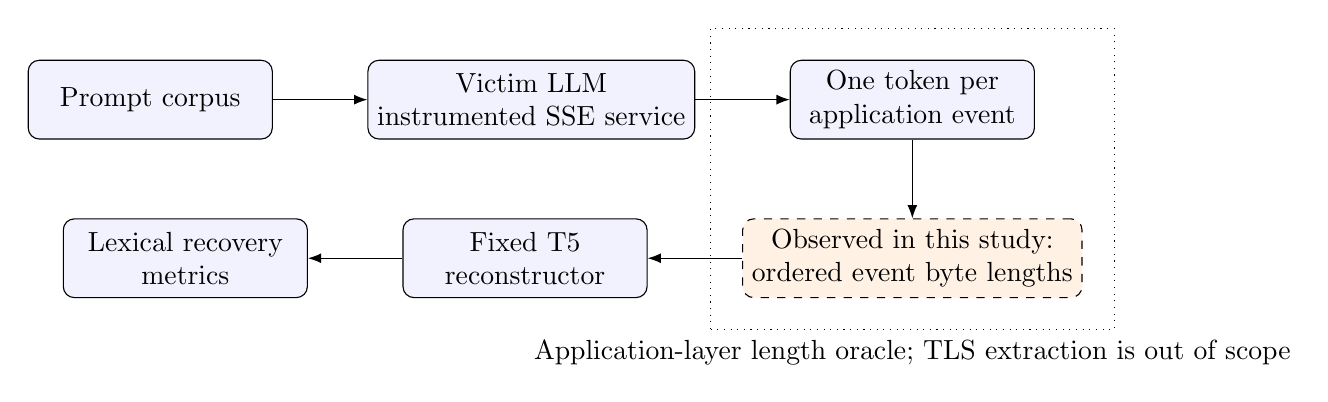
\begin{tikzpicture}[node distance=10mm and 12mm,>=Latex,
box/.style={draw,rounded corners,align=center,minimum height=10mm,minimum width=31mm,fill=blue!5},
obs/.style={draw,dashed,rounded corners,align=center,minimum height=10mm,minimum width=35mm,fill=orange!10}]
\node[box] (user) {Prompt corpus};
\node[box,right=of user] (victim) {Victim LLM\\instrumented SSE service};
\node[box,right=of victim] (stream) {One token per\\application event};
\node[obs,below=of stream] (oracle) {Observed in this study:\\ordered event byte lengths};
\node[box,left=of oracle] (attacker) {Fixed T5\\reconstructor};
\node[box,left=of attacker] (score) {Lexical recovery\\metrics};
\draw[->] (user)--(victim);
\draw[->] (victim)--(stream);
\draw[->] (stream)--(oracle);
\draw[->] (oracle)--(attacker);
\draw[->] (attacker)--(score);
\node[draw,dotted,fit=(stream)(oracle),inner sep=4mm,label=below:{Application-layer length oracle; TLS extraction is out of scope}] {};
\end{tikzpicture}%
}
\caption{Threat model. The experiment begins at SSE-equivalent application-event lengths; it does not claim passive recovery of event boundaries from encrypted transport records.}
\label{fig:threat_model}
\end{figure*}

\subsection{Streaming Harness and Trace Collection}
The measurement harness implemented SSE streaming in a strict one-token-per-event configuration. Each application event followed the format \texttt{data: \textless token\textgreater\textbackslash n\textbackslash n}, while stream termination used \texttt{data: [DONE]\textbackslash n\textbackslash n}. For every emitted token, the harness logged token text for ground-truth evaluation, token UTF-8 length, application-event UTF-8 length, and relative emission timestamp. Per-run metadata additionally included the model identifier, decoding parameters, prompt, generated response text, and token count. The attacker-facing reconstruction input contained lengths only.

Within the experimental harness, this design creates a direct mapping between emitted tokens and recorded SSE-equivalent application events. This mapping enables controlled reconstruction experiments from application-layer length traces. Denoting the UTF-8 length of the $t$-th recorded application event by $L^{\mathrm{event}}_t$, the estimated token length is
\begin{equation}
L^{\mathrm{tok}}_t = L^{\mathrm{event}}_t - 8,
\end{equation}
where 8 bytes correspond to the fixed overhead generated by the prefix \texttt{data: } and suffix \texttt{\textbackslash n\textbackslash n} in the laboratory serialization. This relation applies only to the stated serialization, without additional SSE fields or transformations. The terminal \texttt{[DONE]} event is excluded from reconstruction.

\subsection{Reconstruction Pipeline}
The inversion pipeline follows the sequence-to-text procedure introduced by Weiss \emph{et al.}~\cite{weiss2024prompt}. First, the token-length sequence is segmented heuristically into sentence-like chunks. Second, the initial chunk is decoded using \texttt{royweiss1/T5\_FirstSentences}. Third, subsequent chunks are decoded with \texttt{royweiss1/T5\_MiddleSentences} using preceding context. Finally, multiple decoding candidates are ranked according to aggregate generation confidence represented by the transition log-probability sum.

The reconstruction design is conditional rather than purely tokenwise. Instead of recovering each token independently, it maps length patterns into coherent text spans and uses context to improve linguistic plausibility (Figure~\ref{fig:pipeline}). Our quantitative claims nevertheless concern lexical recovery; semantic correctness was not established by human annotation.

\begin{figure*}[ht]
\centering
\resizebox{\textwidth}{!}{%
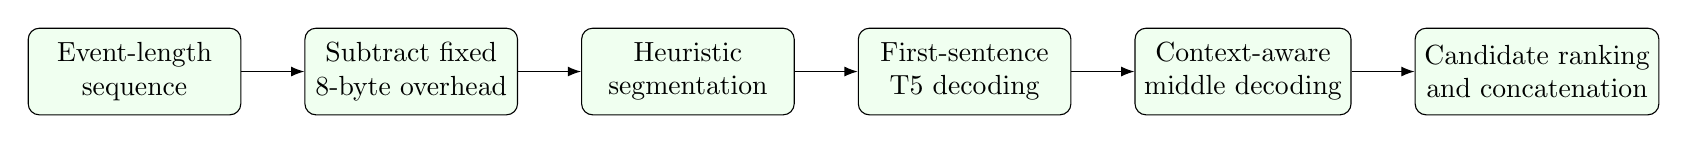
\begin{tikzpicture}[node distance=8mm,>=Latex,
pipelinebox/.style={draw,rounded corners,align=center,minimum height=11mm,minimum width=27mm,fill=green!6}]
\node[pipelinebox] (capture) {Event-length\\sequence};
\node[pipelinebox,right=of capture] (norm) {Subtract fixed\\8-byte overhead};
\node[pipelinebox,right=of norm] (segment) {Heuristic\\segmentation};
\node[pipelinebox,right=of segment] (first) {First-sentence\\T5 decoding};
\node[pipelinebox,right=of first] (middle) {Context-aware\\middle decoding};
\node[pipelinebox,right=of middle] (rank) {Candidate ranking\\and concatenation};
\draw[->] (capture)--(norm);
\draw[->] (norm)--(segment);
\draw[->] (segment)--(first);
\draw[->] (first)--(middle);
\draw[->] (middle)--(rank);
\end{tikzpicture}%
}
\caption{Reconstruction pipeline used for all victim models and defense transformations. The decoder checkpoints and ranking procedure remain fixed.}
\label{fig:pipeline}
\end{figure*}

\subsection{Prompt Corpus and Experimental Protocol}
The synthetic prompt corpus comprised 15 topical files with 20 prompts each, yielding 300 prompts. It covered legal, health-related, financial, employment, and security matters. Prompt scheduling followed a round-robin strategy to reduce topical clustering during data collection.

Victim-model decoding was deterministic, with temperature set to 0.0 and \texttt{top\_p} set to 1.0. For primary cross-model claims, a prespecified standardized subset was selected with the following shared parameters: $N=300$, \texttt{max\_new\_tokens}=512, \texttt{samples\_per\_segment}=3, \texttt{max\_sentences}=0 (reconstruct every heuristic segment), and \texttt{num\_first\_candidates}=3. Six models used the instrumented one-token KV-cache loop. Gemma-2-2B-it used Hugging Face greedy \texttt{model.generate()} because its HybridCache implementation exceeded the 8\,GB laboratory GPU in that loop; decoding parameters remained temperature 0.0 and \texttt{top\_p} 1.0. A sample is marked EOS-complete when generation stopped on an end-of-sequence token before the 512-token budget (\texttt{finish\_reason=eos}, \texttt{response\_complete=true}). Length-truncated samples remain in the primary $N=300$ comparison; EOS-complete subsets are reported separately and are never treated as interchangeable with truncated prefixes.

The evaluated models are listed in Table~\ref{tab:model_metadata}. Six are instruction- or chat-tuned; Phi-1.5 is a base model retained as a stress test and is not used to infer a general base-versus-instruction effect~\cite{qwen25report,llama3report,llama32blog,gemma2report,phi15report,tinyllama2024,phi3report}. A common token budget does not imply a common amount of text across tokenizer families. Table~\ref{tab:length_covariates} reports covariates for the 2100 publication samples. Truncation at 512 tokens ranged from 34.3\% (Llama-3.2-3B) to 100\% (Phi-3.5-mini). Phi-3.5-mini produced no EOS-complete sample at this budget.

\begin{table*}[ht]
\centering
\caption{Victim models used in the standardized comparison. Parameter counts follow the cited model cards and technical reports. Licenses are those published with the Hugging Face checkpoints used in the experiments.}
\label{tab:model_metadata}
\resizebox{\textwidth}{!}{%
\begin{tabular}{l l l l l}
\toprule
Model & Checkpoint & Parameters & License & Tokenizer \\
\midrule
Qwen2.5-1.5B-Instruct & \texttt{Qwen/Qwen2.5-1.5B-Instruct} & 1.54B & Apache 2.0 & Qwen2 \\
Qwen2.5-3B-Instruct & \texttt{Qwen/Qwen2.5-3B-Instruct} & 3.09B & Qwen Research & Qwen2 \\
Llama-3.2-3B-Instruct & \texttt{meta-llama/Llama-3.2-3B-Instruct} & 3.2B & Llama 3.2 Community & Llama 3 \\
Gemma-2-2B-it & \texttt{google/gemma-2-2b-it} & 2.6B & Gemma & Gemma \\
Phi-1.5 & \texttt{microsoft/phi-1\_5} & 1.3B & MIT & CodeGen \\
TinyLlama-1.1B-Chat-v1.0 & \texttt{TinyLlama/TinyLlama-1.1B-Chat-v1.0} & 1.1B & Apache 2.0 & Llama 2 \\
Phi-3.5-mini-instruct & \texttt{microsoft/Phi-3.5-mini-instruct} & 3.8B & MIT & Llama/Phi-3 \\
\bottomrule
\end{tabular}%
}
\end{table*}

\begin{table}[ht]
\centering
\caption{Response-length covariates for the standardized subset ($N=300$ per model). Truncation is the percentage of samples with \texttt{token\_count}$\geq 512$.}
\label{tab:length_covariates}
\resizebox{\columnwidth}{!}{%
\begin{tabular}{l c c c c}
\toprule
Model & Mean tokens & Mean chars & Mean B/token & Trunc. (\%) \\
\midrule
Qwen2.5-1.5B-Instruct & 418.3 & 2069 & 4.91 & 44.3 \\
Qwen2.5-3B-Instruct & 497.6 & 2417 & 4.87 & 83.3 \\
Llama-3.2-3B-Instruct & 431.0 & 2081 & 4.84 & 34.3 \\
Gemma-2-2B-it & 490.6 & 2257 & 4.60 & 74.3 \\
Phi-1.5 & 395.4 & 2035 & 5.11 & 52.0 \\
TinyLlama-1.1B-Chat-v1.0 & 428.3 & 1478 & 3.45 & 41.0 \\
Phi-3.5-mini-instruct & 512.0 & 1755 & 3.43 & 100.0 \\
\bottomrule
\end{tabular}%
}
\end{table}

\subsection{Evaluation Metrics}
Reconstruction quality was computed using four lexical criteria. The reported Levenshtein value is $\texttt{ed\_norm}=d(R,\widehat{R})/|R|$, where character length $|R|$ is the denominator; it can therefore exceed 1 when the reconstruction is much longer than the reference~\cite{levenshtein1966binary}. ROUGE-1 precision and ROUGE-L precision quantify unigram and longest-common-subsequence overlap~\cite{lin2004rouge}. The primary metric, $\phi$, is cosine similarity between unweighted, case-normalized term-frequency vectors of the reference and reconstruction~\cite{salton1975vector}. It was recomputed from stored texts for all 2100 samples to avoid mixing scoring backends.

The study also reports lexical recovery rate $\mathrm{LR}@0.5$, the proportion of samples with $\phi>0.5$. This threshold is a descriptive operating point, not a calibrated success criterion. Neither $\phi$ nor $\mathrm{LR}@0.5$ establishes factual, semantic, or operationally useful reconstruction.

\subsection{Trace-Information Controls}
To separate trace contribution from the reconstructor's language prior, we evaluated four inputs on the same topic-balanced set of 30 prompts for Qwen2.5-1.5B-Instruct and Llama-3.2-3B-Instruct, again using the 96-token pilot traces: (i) the true trace; (ii) the same lengths randomly permuted within the response; (iii) a constant sequence equal to the rounded within-response mean length; and (iv) a length sequence taken from another prompt and cycled to the same number of positions. The shuffled condition preserves the marginal length distribution but destroys order; the constant condition removes length variation; and the cross-prompt condition preserves a plausible trace while breaking prompt alignment. These controls are descriptive pilots and do not estimate mutual information.

\subsection{Statistical Analysis}
Because the same 300 prompts were issued to every model, cross-model inference used prompt-aligned observations. Mean metrics were accompanied by percentile-bootstrap 95\% confidence intervals~\cite{efron1994bootstrap} based on $B=10{,}000$ prompt-index resamples with replacement and seed \texttt{20260706}. Confidence intervals for mean pairwise differences were obtained by bootstrapping within-prompt differences. Wilson 95\% intervals were used for $\mathrm{LR}@0.5$. These intervals quantify variation over the prompt set and do not include uncertainty from repeated victim generations. Decoder-seed uncertainty is reported separately for a two-model subset (Section~\ref{sec:robustness-methods}).

Pairwise differences in per-prompt $\phi$ were assessed using two-sided paired Wilcoxon signed-rank tests~\cite{wilcoxon1945individual}. Absolute nonzero differences received average ranks when tied; exact zero differences were removed under the Wilcoxon convention. The implementation applied the standard tie correction to the normal-approximation variance and a continuity correction of 0.5. The effective $n$ was 300 for 20 pairs and 299 for TinyLlama versus Phi-3.5-mini. Holm--Bonferroni correction controlled family-wise error over all $\binom{7}{2}=21$ model pairs~\cite{holm1979simple}, and rank-biserial correlation quantified effect size. Defense--baseline comparisons used the same paired procedure with Holm correction over ten tests. Statistical significance was defined as adjusted $p<0.05$.

\subsection{Defense Evaluation Protocol}
Five configurations were evaluated on the same 30 topic-balanced prompts for each of Qwen2.5-1.5B-Instruct and Llama-3.2-3B-Instruct, using earlier 96-token traces rather than the 512-token primary campaign. Let $\ell_t$ denote token-payload length after the fixed eight-byte laboratory SSE overhead has been removed.
\begin{itemize}[leftmargin=2em]
    \item \texttt{bucket\_8}: replace $\ell_t$ by $8\lceil \ell_t/8\rceil$, independently and online for every event.
    \item \texttt{pad\_32}: replace each token-length observation by a constant 32-byte protected unit. The largest token in the evaluated subset occupied 16 UTF-8 bytes, so every token fit within the unit.
    \item \texttt{batch\_2} and \texttt{batch\_4}: concatenate the lengths of consecutive groups of two or four tokens into one attacker-visible value. The final incomplete group, if present, is retained.
    \item \texttt{rand\_pad\_8}: add an independently sampled integer $U_t\sim\mathrm{Uniform}\{0,\ldots,8\}$ using a recorded deterministic seed.
\end{itemize}
The transformed sequences were passed directly to the same segmentation and decoding pipeline. The reconstructor was frozen and was not retrained or calibrated on defended traces. We report recovery-score reduction as $100(1-\bar\phi_d/\bar\phi_0)$. Payload-size overhead compares the sum of transformed units with the sum of original token bytes. This deliberately narrow accounting excludes SSE syntax, transport headers, packetization, buffering delay, and user-perceived latency. Batching has zero overhead only under this payload-sum definition; its reduction in observable frame count is reported separately.

\subsection{Repeated Decoder Seeds and Adaptive Attacker}\label{sec:robustness-methods}
The primary seven-model table uses one reconstructor draw per sample. Decoder-seed uncertainty and a defense-aware attacker were evaluated on the 512-token traces of Qwen2.5-1.5B-Instruct and Llama-3.2-3B-Instruct. Two prompts were taken from each of the 15 topics ($n=30$ test prompts per model). The remaining 270 traces of each model formed a prompt-disjoint calibration set. An EOS-complete-only split would have left 137 (Qwen) and 167 (Llama) calibration traces, below the prespecified minimum of 200, and was therefore not used. Of the 30 test prompts, 24 (Qwen) and 21 (Llama) were EOS-complete.

Reconstruction was repeated for five decoder seeds, \texttt{20260706}--\texttt{20260710}. For a given prompt the same decoder seed was used in every defense and attacker condition (common random numbers). The seed is derived by BLAKE2s over $(\texttt{decoder}, \text{seed index}, \text{prompt idx})$ and does not depend on \texttt{PYTHONHASHSEED}. Mean $\phi$ is reported with a crossed bootstrap 95\% confidence interval that resamples the prompt axis and the seed axis independently ($B=10{,}000$). Between-seed variation is the sample standard deviation of the five seed-specific means; seed repeats are not treated as independent prompts. Robustness reconstructions used one stochastic first-sentence T5 sample per seed. The seven-model primary table reconstructs every available segment with three samples per segment.

The adaptive attacker is a prompt-disjoint empirical MAP inverse of each defense, followed by the unchanged T5 decoder. It learns the empirical distribution of clean token lengths (or, for batching, of length tuples) conditional on the defended observation from the 270 calibration traces of the same victim model. Test responses are never used for fitting. This is a calibrated length inverse, not end-to-end T5 retraining. Baseline traces are scored with the frozen reconstructor only. Each of the five transformations is scored with both the frozen reconstructor and the MAP inverse. The design comprises 22 complete cells and 3300 reconstructions. A run is admitted to the manuscript table only when \texttt{robustness\_eval.json} reports \texttt{complete: true}.

\subsection{Run Completeness Criteria}
A run was considered complete only if all required artifacts were present (\texttt{config.json}, \texttt{progress.json}, \texttt{samples.jsonl}, \texttt{summary.json}, \texttt{summary.md}, and \texttt{summary\_by\_topic.csv}) and internal counts matched exactly:
\begin{equation}
\texttt{progress.done}=\texttt{progress.total}=\texttt{summary.count}=\texttt{lines(samples.jsonl)}.
\end{equation}
These checks were applied before including any run in the main comparative analysis.

\subsection{Reproducibility Artifacts}
All experimental materials required to reproduce the reported tables and figures are released in the public repository at \url{https://github.com/jackaugustyn/LLeakM}. The package includes the instrumented SSE server, the reconstruction pipeline, the 300-prompt corpus, per-sample outputs for the seven standardized runs, defense and trace-baseline results, analysis scripts, and a SHA-256 manifest under \texttt{experiment\_validation/}.

\section{Results}
All seven standardized 512-token runs passed the completeness checks and contributed 300 aligned prompts, for 2100 primary samples. Four findings organize the results. First, the true trace outperformed all three control traces in both 96-token pilot models. Second, transfer of the fixed reconstructor on the 512-token campaign split into a high-$\phi$ cluster of five models and a near-floor pair. Third, every tested framing transformation lowered the frozen reconstructor's mean score on the 96-token pilots, but those score reductions should not be interpreted as reductions in mutual information. Fourth, five decoder seeds and a prompt-disjoint MAP inverse on 512-token traces of two models showed that seed-to-seed SD is small relative to defense effects, that the MAP inverse recovers most frozen losses on bucketing and batching, and that it does not restore the inflated frozen score of \texttt{pad\_32}.

\subsection{Trace Contribution versus Language Prior}
Table~\ref{tab:trace_controls} shows that the reconstructor retained nonzero lexical overlap when the trace was destroyed or mismatched. For Qwen2.5-1.5B, the true-trace mean was 0.302, compared with 0.209 for shuffled lengths, 0.107 for a constant trace, and 0.256 for a cross-prompt trace. The corresponding Llama means were 0.291, 0.187, 0.124, and 0.231. The true trace therefore improved mean $\phi$ over the three controls by 0.046--0.196 for Qwen and 0.060--0.167 for Llama. The gap relative to shuffled traces indicates that order matters; the nonzero control scores show that generic lexical overlap and the reconstructor's language prior also contribute materially.

\begin{table}[ht]
\centering
\caption{Trace-information controls on the topic-balanced pilot ($n=30$ prompts per model and condition). Intervals are percentile-bootstrap 95\% confidence intervals for the mean.}
\label{tab:trace_controls}
\resizebox{\columnwidth}{!}{%
\begin{tabular}{l l c c c}
\toprule
Model & Trace & Mean $\phi$ & 95\% CI & Difference from true \\
\midrule
Qwen2.5-1.5B & true & 0.3024 & [0.2607, 0.3457] & -- \\
 & shuffled & 0.2091 & [0.1734, 0.2463] & $-0.0933$ \\
 & constant & 0.1068 & [0.0844, 0.1303] & $-0.1957$ \\
 & cross-prompt & 0.2561 & [0.2296, 0.2837] & $-0.0463$ \\
\midrule
Llama-3.2-3B & true & 0.2913 & [0.2568, 0.3282] & -- \\
 & shuffled & 0.1872 & [0.1623, 0.2119] & $-0.1041$ \\
 & constant & 0.1242 & [0.0981, 0.1529] & $-0.1671$ \\
 & cross-prompt & 0.2312 & [0.2010, 0.2618] & $-0.0601$ \\
\bottomrule
\end{tabular}%
}
\end{table}

\subsection{Cross-Model Comparison under Standardized Conditions}
Table~\ref{tab:main_results} reports the primary comparison, and Figure~\ref{fig:model_ci} displays the mean-score intervals. Mean $\phi$ split into two groups. Qwen2.5-1.5B-Instruct, Qwen2.5-3B-Instruct, Phi-1.5, Llama-3.2-3B-Instruct, and Gemma-2-2B-it formed a high-overlap cluster with mean $\phi$ from 0.5170 to 0.5680 and $\mathrm{LR}@0.5$ from 59.67\% to 76.33\%. TinyLlama-1.1B-Chat (0.0302) and Phi-3.5-mini-instruct (0.0434) remained at the floor, with no sample above $\phi>0.5$. Phi-1.5 is a base-model stress test, so its position in the high cluster does not support a base-versus-instruction claim. ROUGE-1 precision in the high cluster (0.2329--0.3149) is much closer across models than $\phi$ and remains far below what a readable paraphrase would require.

\begin{table*}[ht]
\centering
\caption{Primary cross-model comparison using one term-frequency cosine implementation for all samples ($N=300$ per model, 512-token budget).}
\label{tab:main_results}
\resizebox{\textwidth}{!}{%
\begin{tabular}{l l c c c c c}
\toprule
Model & Type & $\phi_{\mathrm{mean}}$ & $ed_{\mathrm{norm}}$ & R1 Precision & RL Precision & $\mathrm{LR}@0.5$ \\
\midrule
Qwen2.5-1.5B-Instruct & instruct & 0.5680 & 0.6841 & 0.3149 & 0.1962 & 76.33\% \\
Qwen2.5-3B-Instruct & instruct & 0.5521 & 0.7336 & 0.2748 & 0.1423 & 70.67\% \\
Phi-1.5 & base & 0.5383 & 0.7645 & 0.2775 & 0.1703 & 65.33\% \\
Llama-3.2-3B-Instruct & instruct & 0.5360 & 0.7312 & 0.2668 & 0.1445 & 68.33\% \\
Gemma-2-2B-it & instruct & 0.5170 & 0.8428 & 0.2329 & 0.1151 & 59.67\% \\
Phi-3.5-mini-instruct & instruct & 0.0434 & 0.9931 & 0.0161 & 0.0117 & 0.00\% \\
TinyLlama-1.1B-Chat-v1.0 & chat & 0.0302 & 0.9814 & 0.0158 & 0.0119 & 0.00\% \\
\bottomrule
\end{tabular}%
}
\end{table*}

\begin{figure*}[ht]
\centering
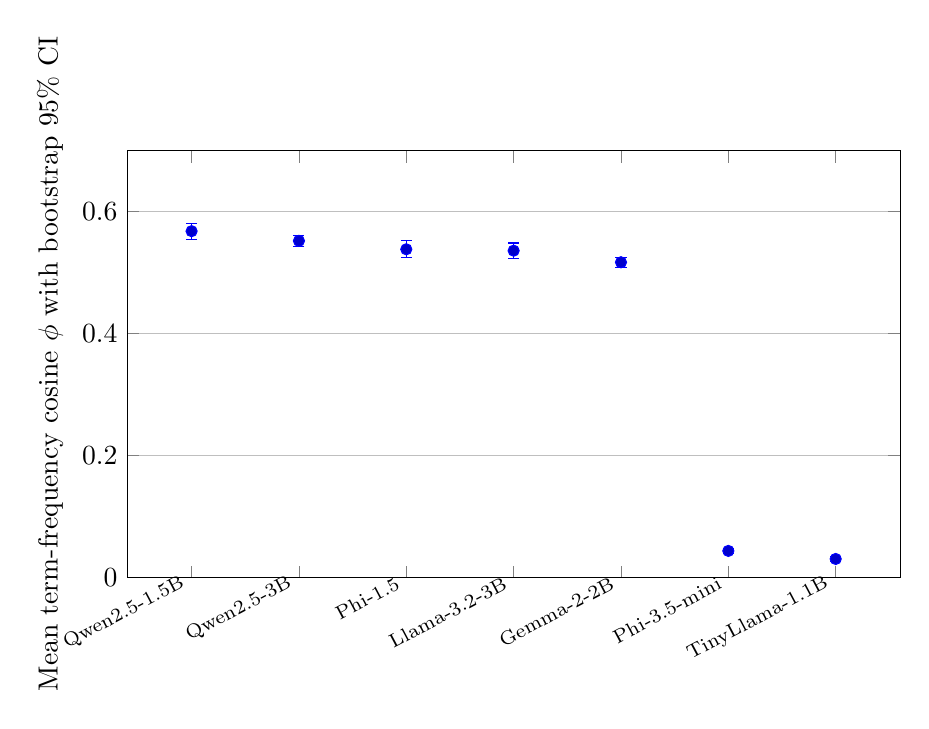
\begin{tikzpicture}
\begin{axis}[width=0.94\textwidth,height=7cm,ymin=0,ymax=0.70,
ylabel={Mean term-frequency cosine $\phi$ with bootstrap 95\% CI},
symbolic x coords={Qwen1.5,Qwen3,Phi1.5,Llama3,Gemma2,Phi3.5,TinyLlama},xtick=data,
xticklabels={Qwen2.5-1.5B,Qwen2.5-3B,Phi-1.5,Llama-3.2-3B,Gemma-2-2B,Phi-3.5-mini,TinyLlama-1.1B},
x tick label style={rotate=28,anchor=east,font=\scriptsize},ymajorgrids]
\addplot+[only marks,mark=*,blue,error bars/.cd,y dir=both,y explicit]
coordinates {(Qwen1.5,0.5680) +- (0,0.0130) (Qwen3,0.5521) +- (0,0.0094)
(Phi1.5,0.5383) +- (0,0.0138) (Llama3,0.5360) +- (0,0.0126)
(Gemma2,0.5170) +- (0,0.0084) (Phi3.5,0.0434) +- (0,0.0043)
(TinyLlama,0.0302) +- (0,0.0038)};
\end{axis}
\end{tikzpicture}
\caption{Mean lexical reconstruction score and bootstrap 95\% confidence intervals for the seven standardized 512-token runs. Error-bar half-widths are rounded to four decimals for visualization; asymmetric endpoints are reported in Table~\ref{tab:statistical_results}.}
\label{fig:model_ci}
\end{figure*}

All reported $\phi$ values were recomputed from stored text. This step matters because stored per-run scores mixed MiniLM and term-frequency backends; no historical per-run score is used in the analysis.

\subsection{Completeness: All Samples versus EOS-Only}
Table~\ref{tab:eos_completeness} compares the primary $N=300$ scores with the EOS-complete subset. EOS rates ranged from 0.0\% (Phi-3.5-mini) to 65.7\% (Llama-3.2-3B). Restricting to complete answers does not systematically raise $\phi$: Qwen2.5-3B rises from 0.5521 to 0.5936 ($n=50$), whereas Phi-1.5 falls from 0.5383 to 0.5028 ($n=144$). Phi-3.5-mini has no complete-answer subset at this budget, so it is excluded from EOS-only claims.

\begin{table*}[ht]
\centering
\caption{EOS completeness versus the full $N=300$ set. Complete-only $\phi$ and $\mathrm{LR}@0.5$ use \texttt{response\_complete} samples only. Phi-3.5-mini has $n_{\mathrm{EOS}}=0$.}
\label{tab:eos_completeness}
\resizebox{\textwidth}{!}{%
\begin{tabular}{l c c c c c c c}
\toprule
Model & $n_{\mathrm{EOS}}$ & EOS (\%) & Trunc.\ (\%) & $\phi$ all & $\phi$ EOS & $\mathrm{LR}$ all & $\mathrm{LR}$ EOS \\
\midrule
Qwen2.5-1.5B-Instruct & 167 & 55.7 & 44.3 & 0.5680 & 0.5857 & 76.33 & 78.44 \\
Qwen2.5-3B-Instruct & 50 & 16.7 & 83.3 & 0.5521 & 0.5936 & 70.67 & 90.00 \\
Phi-1.5 & 144 & 48.0 & 52.0 & 0.5383 & 0.5028 & 65.33 & 51.39 \\
Llama-3.2-3B-Instruct & 197 & 65.7 & 34.3 & 0.5360 & 0.5203 & 68.33 & 62.94 \\
Gemma-2-2B-it & 77 & 25.7 & 74.3 & 0.5170 & 0.5090 & 59.67 & 53.25 \\
Phi-3.5-mini-instruct & 0 & 0.0 & 100.0 & 0.0434 & -- & 0.00 & -- \\
TinyLlama-1.1B-Chat & 177 & 59.0 & 41.0 & 0.0302 & 0.0297 & 0.00 & 0.00 \\
\bottomrule
\end{tabular}%
}
\end{table*}

\subsection{Statistical Uncertainty and Pairwise Tests}
Table~\ref{tab:statistical_results} adds uncertainty intervals. 17 of 21 paired cross-model comparisons remained significant after Holm correction. The four non-significant pairs all lie inside the high-$\phi$ cluster: Qwen2.5-1.5B versus Qwen2.5-3B (mean paired difference 0.0160, bootstrap 95\% CI $[0.0020,0.0303]$, rank-biserial $r=0.149$, $p_{\mathrm{Holm}}=0.1023$); Qwen2.5-3B versus Llama-3.2-3B (0.0161, 95\% CI $[0.0021,0.0305]$, $r=0.116$, $p_{\mathrm{Holm}}=0.2470$); Qwen2.5-3B versus Phi-1.5 (0.0138, 95\% CI $[-0.0012,0.0287]$, $r=0.079$, $p_{\mathrm{Holm}}=0.4765$); and Llama-3.2-3B versus Phi-1.5 ($-0.0022$, 95\% CI $[-0.0199,0.0159]$, $r=-0.009$, $p_{\mathrm{Holm}}=0.8960$). Qwen2.5-1.5B versus TinyLlama differed by 0.5378 ($r=1.000$, $p_{\mathrm{Holm}}<0.0001$). These tests address prompt-sampling variation, not causal model effects or decoder-seed variability.

For the six instruction/chat models ($n=1800$), model indicators alone gave $R^2=0.897$. Response characters, mean token bytes, and truncation alone gave $R^2=0.749$, while the combined specification gave $R^2=0.904$. Adding the measured length covariates therefore changed $R^2$ by only 0.007 beyond model indicators in this dataset.

\begin{table*}[ht]
\centering
\caption{Uncertainty-aware results. Mean-$\phi$ intervals use 10,000 bootstrap resamples; $\mathrm{LR}@0.5$ intervals are Wilson 95\% intervals.}
\label{tab:statistical_results}
\begin{tabular}{l c c c c}
\toprule
Model & Mean $\phi$ & 95\% CI & $\mathrm{LR}@0.5$ & 95\% CI \\
\midrule
Qwen2.5-1.5B-Instruct & 0.5680 & [0.5551, 0.5810] & 76.33\% & [71.21, 80.79]\% \\
Qwen2.5-3B-Instruct & 0.5521 & [0.5427, 0.5615] & 70.67\% & [65.28, 75.53]\% \\
Phi-1.5 & 0.5383 & [0.5244, 0.5516] & 65.33\% & [59.78, 70.49]\% \\
Llama-3.2-3B-Instruct & 0.5360 & [0.5234, 0.5483] & 68.33\% & [62.87, 73.34]\% \\
Gemma-2-2B-it & 0.5170 & [0.5089, 0.5254] & 59.67\% & [54.03, 65.06]\% \\
Phi-3.5-mini-instruct & 0.0434 & [0.0393, 0.0477] & 0.00\% & [0.00, 1.26]\% \\
TinyLlama-1.1B-Chat & 0.0302 & [0.0267, 0.0340] & 0.00\% & [0.00, 1.26]\% \\
\bottomrule
\end{tabular}
\end{table*}

\subsection{What the Lexical Scores Represent}
The score range is easier to interpret from examples (Table~\ref{tab:qualitative_examples}). At $\phi=0.972$, the Qwen reconstruction copied the template almost verbatim but substituted ``physical health'' for ``drinking habits''. At $\phi=0.698$, the Gemma reconstruction retained relationship-related vocabulary while changing the advice. At $\phi=0.570$, a Qwen sample above the descriptive 0.5 threshold was topically wrong. These cases confirm that $\phi$ is useful for consistent aggregate comparison but cannot replace human assessment of disclosure severity.

\begin{table*}[ht]
\centering
\caption{Post hoc examples illustrating the meaning of $\phi$. Excerpts are truncated for space and are not prevalence estimates.}
\label{tab:qualitative_examples}
\begin{tabularx}{\textwidth}{l c X X}
\toprule
Model & $\phi$ & Reference excerpt & Reconstruction excerpt \\
\midrule
Qwen2.5-1.5B & 0.972 & If you are concerned about your drinking habits, it is important to seek help from a healthcare professional. They can provide you with a diagnosis and treatment plan that is tailored to your specific needs. & If you are concerned about your physical health, it is important to seek help from a healthcare professional. They can provide you with a diagnosis and treatment plan that is tailored to your specific needs. \\
Gemma-2-2B & 0.698 & It's understandable to feel hurt and betrayed when you discover lies in a relationship. Trust is the foundation of any healthy relationship, and its breach can be incredibly damaging. & Yes, 2 compatibility is more than one compatibility that can increase risk in a relationship. While it can contribute to the overall relationship, the two should not be considered separate. \\
Qwen2.5-1.5B & 0.570 & When you are pressured to sign a contract you do not understand, it's important to document evidence to protect your rights. & Here are the locations in Bali (excluding Bali to the south) as a directory of monuments dedicated to various holy places. \\
\bottomrule
\end{tabularx}
\end{table*}

\subsection{Framing Transformations against the Frozen Reconstructor}\label{sec:defense}
Every transformation lowered mean $\phi$ (Table~\ref{tab:defense_results}), and all ten paired defense--baseline comparisons remained significant after Holm correction. The largest observed score reduction was 90.3\% for \texttt{bucket\_8} on Qwen; the smallest was 35.0\% for \texttt{pad\_32} on Llama. Batching by two or four reduced the score by 67.7--69.2\% while reducing the visible frame count to 48 or 24. Figure~\ref{fig:defense_tradeoff} plots the narrow payload-overhead measure against score reduction.

The apparent ordering is not a privacy ranking. In particular, \texttt{pad\_32} removes per-token length variation more completely than bucketing, yet it leaves a higher lexical score because a constant sequence of 32s drives the frozen decoder toward generic text that overlaps the references. The residual score therefore contains language-prior overlap and decoder behavior, not just information remaining in the trace.

\begin{table*}[ht]
\centering
\caption{Framing transformations against the frozen, non-adaptive reconstructor ($n=30$ paired prompts per model). Overhead is computed on protected token-payload units and excludes SSE syntax, transport headers, buffering delay, and latency.}
\label{tab:defense_results}
\resizebox{\textwidth}{!}{%
\begin{tabular}{l l c c c c c}
\toprule
Model & Defense & Mean $\phi$ & 95\% CI & Score reduction & Payload overhead & Frames \\
\midrule
Qwen2.5-1.5B & baseline & 0.3010 & [0.2537, 0.3508] & -- & 0.0\% & 96 \\
 & bucket\_8 & 0.0293 & [0.0198, 0.0397] & 90.3\% & 82.4\% & 96 \\
 & pad\_32 & 0.1901 & [0.1667, 0.2150] & 36.8\% & 538.0\% & 96 \\
 & batch\_2 & 0.0928 & [0.0791, 0.1072] & 69.2\% & 0.0\% & 48 \\
 & batch\_4 & 0.0950 & [0.0668, 0.1269] & 68.4\% & 0.0\% & 24 \\
 & rand\_pad\_8 & 0.1033 & [0.0871, 0.1203] & 65.7\% & 78.5\% & 96 \\
\midrule
Llama-3.2-3B & baseline & 0.2576 & [0.2177, 0.2978] & -- & 0.0\% & 96 \\
 & bucket\_8 & 0.0428 & [0.0305, 0.0563] & 83.4\% & 88.6\% & 96 \\
 & pad\_32 & 0.1674 & [0.1382, 0.2003] & 35.0\% & 565.1\% & 96 \\
 & batch\_2 & 0.0823 & [0.0684, 0.0967] & 68.0\% & 0.0\% & 48 \\
 & batch\_4 & 0.0832 & [0.0615, 0.1055] & 67.7\% & 0.0\% & 24 \\
 & rand\_pad\_8 & 0.1004 & [0.0834, 0.1186] & 61.0\% & 81.9\% & 96 \\
\bottomrule
\end{tabular}%
}
\end{table*}

\begin{figure}[ht]
\centering
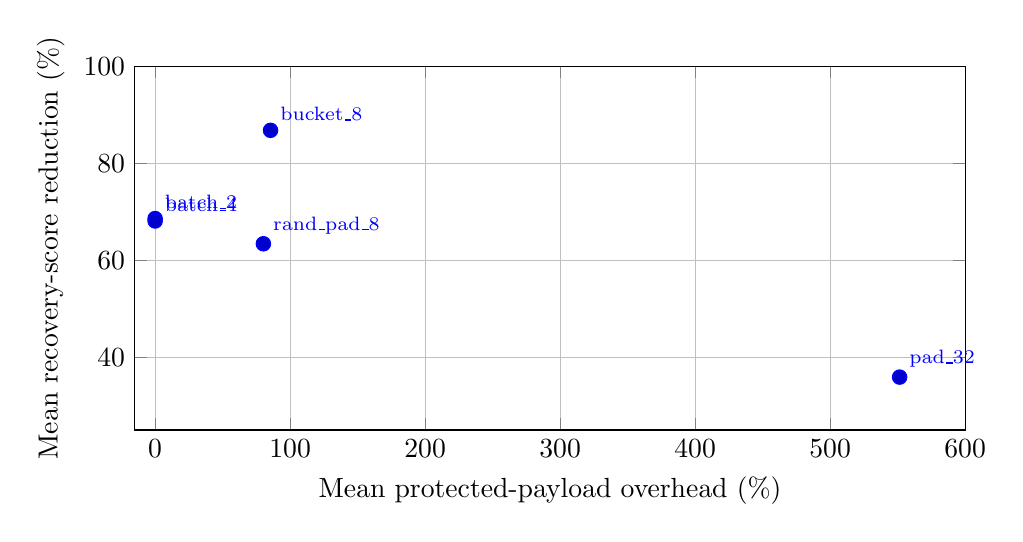
\begin{tikzpicture}
\begin{axis}[width=\columnwidth,height=6.2cm,xmin=-15,xmax=600,ymin=25,ymax=100,
xlabel={Mean protected-payload overhead (\%)},ylabel={Mean recovery-score reduction (\%)},grid=major,
nodes near coords,point meta=explicit symbolic,every node near coord/.append style={font=\scriptsize,anchor=south west}]
\addplot+[only marks,mark=*,mark size=2.6pt,blue]
coordinates {(85.5,86.8) [bucket\_8] (551.5,35.9) [pad\_32]
(0,68.6) [batch\_2] (0,68.1) [batch\_4] (80.2,63.4) [rand\_pad\_8]};
\end{axis}
\end{tikzpicture}
\caption{Recovery-score reduction versus protected-payload overhead, averaged over the two pilot models. Batching overlaps at zero payload-sum overhead but changes frame count and latency. The plot characterizes one frozen reconstructor, not information-theoretic privacy.}
\label{fig:defense_tradeoff}
\end{figure}

No defended model--configuration pair produced a sample above $\phi>0.5$. A zero count among 30 observations still has a Wilson 95\% upper bound of 11.4\%, so the pilot does not establish zero residual risk. It shows only that the tested transformations hindered this non-adaptive reconstructor.

\subsection{Decoder-Seed Repeats and the MAP Inverse}\label{sec:robustness}
Table~\ref{tab:robustness} reports the 22 complete cells ($n=30$ prompts, five seeds, 150 reconstructions per cell). Baseline first-sentence mean $\phi$ was 0.1988 for Qwen2.5-1.5B and 0.1860 for Llama-3.2-3B. Between-seed SDs of cell means ranged from 0.0032 to 0.0184, small relative to the frozen defense drops. Common random numbers were used across conditions of each prompt.

Against the frozen first-sentence decoder, \texttt{bucket\_8} produced the largest score reductions (78.8\% Qwen, 69.4\% Llama). Batching reduced mean $\phi$ by 36.8--49.5\%. Randomized padding reduced it by 37.5\% and 43.8\%. Fixed-width \texttt{pad\_32} increased mean $\phi$ relative to baseline (signed reductions $-19.2\%$ and $-22.1\%$): a constant sequence of 32s drives the decoder toward generic text that overlaps the references, as in the 96-token pilot.

The prompt-disjoint MAP inverse recovered most of those frozen losses for bucketing and batching. For \texttt{bucket\_8} the adaptive means (0.2167 and 0.2075) met or exceeded the frozen baselines. Adaptive \texttt{batch\_2} likewise exceeded baseline. Adaptive \texttt{batch\_4} was near baseline for Qwen (signed reduction $2.8\%$) and well above baseline for Llama ($-53.4\%$). Adaptation did not restore the inflated frozen \texttt{pad\_32} score: the MAP inverse of a constant-32 sequence lowered mean $\phi$ to 0.1583 and 0.1492 (reductions 20.4\% and 19.7\% versus baseline). Adaptive \texttt{rand\_pad\_8} recovered part of the frozen drop but remained below baseline (8.8\% and 19.3\%). These recoveries are properties of an empirical length inverse plus the unchanged T5 decoder, not of end-to-end retraining on defended traces.

\begin{table*}[ht]
\centering
\caption{Five-seed, prompt-disjoint MAP evaluation on 512-token traces ($n=30$ prompts per model; 150 reconstructions per cell). Intervals are crossed bootstrap 95\% CIs over prompts and seeds. SD is the standard deviation of the five seed-specific means. Score reduction is $100(1-\bar\phi/\bar\phi_{\mathrm{baseline}})$; negative values mean the cell exceeded the frozen baseline.}
\label{tab:robustness}
\resizebox{\textwidth}{!}{%
\begin{tabular}{l l l c c c c}
\toprule
Model & Defense & Attacker & Mean $\phi$ & 95\% CI & Seed SD & Reduction (\%) \\
\midrule
Qwen2.5-1.5B & baseline & frozen & 0.1988 & [0.1695, 0.2306] & 0.0090 & 0.0 \\
 & bucket\_8 & frozen & 0.0422 & [0.0347, 0.0500] & 0.0040 & 78.8 \\
 & bucket\_8 & adaptive & 0.2167 & [0.1934, 0.2401] & 0.0042 & $-9.0$ \\
 & pad\_32 & frozen & 0.2371 & [0.2109, 0.2633] & 0.0088 & $-19.2$ \\
 & pad\_32 & adaptive & 0.1583 & [0.1349, 0.1837] & 0.0093 & 20.4 \\
 & batch\_2 & frozen & 0.1200 & [0.1057, 0.1357] & 0.0070 & 39.7 \\
 & batch\_2 & adaptive & 0.2380 & [0.2119, 0.2671] & 0.0184 & $-19.7$ \\
 & batch\_4 & frozen & 0.1004 & [0.0800, 0.1241] & 0.0165 & 49.5 \\
 & batch\_4 & adaptive & 0.1932 & [0.1639, 0.2223] & 0.0123 & 2.8 \\
 & rand\_pad\_8 & frozen & 0.1242 & [0.1030, 0.1453] & 0.0035 & 37.5 \\
 & rand\_pad\_8 & adaptive & 0.1813 & [0.1556, 0.2071] & 0.0067 & 8.8 \\
\midrule
Llama-3.2-3B & baseline & frozen & 0.1860 & [0.1594, 0.2129] & 0.0150 & 0.0 \\
 & bucket\_8 & frozen & 0.0569 & [0.0475, 0.0671] & 0.0032 & 69.4 \\
 & bucket\_8 & adaptive & 0.2075 & [0.1819, 0.2342] & 0.0165 & $-11.6$ \\
 & pad\_32 & frozen & 0.2270 & [0.2023, 0.2529] & 0.0067 & $-22.1$ \\
 & pad\_32 & adaptive & 0.1492 & [0.1278, 0.1728] & 0.0035 & 19.7 \\
 & batch\_2 & frozen & 0.0999 & [0.0860, 0.1154] & 0.0091 & 46.3 \\
 & batch\_2 & adaptive & 0.2139 & [0.1827, 0.2442] & 0.0046 & $-15.0$ \\
 & batch\_4 & frozen & 0.1175 & [0.1001, 0.1355] & 0.0052 & 36.8 \\
 & batch\_4 & adaptive & 0.2852 & [0.2517, 0.3204] & 0.0145 & $-53.4$ \\
 & rand\_pad\_8 & frozen & 0.1044 & [0.0862, 0.1240] & 0.0072 & 43.8 \\
 & rand\_pad\_8 & adaptive & 0.1500 & [0.1233, 0.1780] & 0.0075 & 19.3 \\
\bottomrule
\end{tabular}%
}
\end{table*}

\section{Discussion}
\subsection{Evidence of Trace-Dependent Recovery}
The no-signal controls change the interpretation of the main scores. Constant and shuffled sequences still produced nonzero overlap, so the reconstructor can obtain part of its score from generic language patterns. The true traces nevertheless improved mean $\phi$ in both pilot models. This is evidence of exploitable trace dependence for the evaluated algorithm, not a numerical estimate of $I(R;X)$. Establishing an information-theoretic leakage rate would require a defined response alphabet or feature variable, repeated samples, and an appropriate mutual-information estimator or hypothesis-testing framework.

\subsection{Why Transfer Differs across Victim Models}
The seven-model ranking measures compatibility with one fixed reconstructor. Tokenizer vocabularies, whitespace handling, response style, refusal behavior, token-byte distributions, and similarity to the reconstructor's training domain can all affect recovery. The extreme result for Phi-3.5-mini also coincides with output formatting in which many spaces are absent, illustrating that preprocessing and serialization may dominate apparent model effects. The current design does not isolate those mechanisms. It therefore supports a transferability claim, not the statement that one victim model is intrinsically more vulnerable than another.

Topic-level means (exploratory) ranged from 0.6123 (Llama-3.2-3B, legal\_issues) to 0.4768 (safety\_security) within that model; Gemma-2-2B from 0.5571 (personal\_identity) to 0.4778 (financial\_status); and Phi-3.5-mini from 0.0845 (physical\_health) to 0.0280 (beliefs\_values). These ranges do not overturn the two-cluster model ranking.

\subsection{Practical Exploitability}
High bag-of-words overlap was common in the high-$\phi$ cluster: the strongest model had $\mathrm{LR}@0.5=76.33\%$. That rate should not be read as a disclosure rate. ROUGE-1 precision for the same model is 0.3149, and the qualitative examples show that $\phi>0.5$ can coexist with a substituted entity or a wrong topic. Practical harm may still arise from partial phrases, entities, refusals, or topic cues, but those outcomes were not measured. A production-facing claim requires passive extraction of observables from encrypted traffic, a task-specific disclosure metric, and an attacker calibrated to the target service.

Attack efficacy, transport observability, and mitigation efficacy are separate quantities. This distinction also explains the fixed-width result: a generic decoder output may overlap the reference even when the transformed trace has almost no within-response length variation. A prompt-disjoint MAP inverse recovered frozen losses on bucketing and batching without T5 retraining, and it reduced rather than restored the inflated \texttt{pad\_32} frozen score. End-to-end fine-tuning of T5 on defended traces remains a separate experiment. Future studies should include blinded human judgments, entity recovery, topic disclosure, and a fixed paraphrase-aware metric.

\subsection{Limitations}
The study has eight principal limitations. First, it begins with an application-layer length oracle and does not recover event boundaries from TLS, HTTP/2, or QUIC. Second, victim generation was deterministic. The primary seven-model table uses one reconstructor draw per sample; five-seed variation was measured only for two models, 30 prompts, and first-sentence reconstructions. The 96-token control and defense pilots use recorded condition-specific seeds rather than common random numbers. Third, truncation at 512 tokens ranged from 34.3\% to 100\%, and Phi-3.5-mini produced no EOS-complete sample, so complete-answer claims are model-specific. Fourth, $\phi$, ROUGE precision, and reference-normalized edit distance measure lexical overlap, not semantic fidelity or actionable disclosure; term-frequency cosine on long reconstructions can be high when common words overlap. Fifth, trace controls and the 96-token defense pilot cover only two models and 30 prompts per model. The five-seed MAP study uses the same two models on 512-token traces but decodes only the first heuristic segment. Sixth, the adaptive attacker is a prompt-disjoint empirical MAP inverse plus the unchanged T5 decoder, not end-to-end retraining on defended traces. Seventh, payload overhead omits SSE syntax, transport headers, latency, and user-experience costs. Eighth, Gemma-2-2B-it used Hugging Face \texttt{generate()} rather than the one-token loop used for the other six models. These limitations rule out claims of deployment-scale attack success or information-theoretic security.

\subsection{Ethical Considerations}
The study used synthetic prompts and locally generated responses; it did not intercept user traffic or process identifiable personal data. The artifact release is intended to support defensive evaluation of streaming implementations. Deployment testing should use authorized systems, controlled accounts, and coordinated disclosure when a service-specific weakness is found.

\section{Conclusions}
Under a token-granular application-length oracle and a 512-token budget, the fixed reconstructor achieved mean lexical cosine scores from 0.030 to 0.568 across seven victim models. Five models clustered at 0.517--0.568; TinyLlama and Phi-3.5-mini remained near the floor. True traces outperformed shuffled, constant, and cross-prompt controls in two 30-prompt pilots, indicating that the ordered lengths contributed to recovery beyond the decoder's language prior. Model-to-model differences were large, but they measure transfer of this reconstructor rather than intrinsic vulnerability. High $\mathrm{LR}@0.5$ in the upper cluster should be read with ROUGE-1 precision and the qualitative examples: bag-of-words cosine is not a disclosure metric.

All five framing configurations reduced the frozen attacker's mean score by 35.0--90.3\% on the 96-token pilots. On 512-token traces, five decoder seeds changed cell means by SDs of 0.003--0.018, and a prompt-disjoint MAP inverse recovered most frozen losses on bucketing and batching without restoring the inflated \texttt{pad\_32} frozen score. Those results are algorithm-specific stress tests, not proof of information-theoretic protection. The next necessary experiment is an end-to-end, transport-captured evaluation with disclosure-oriented human or task metrics and, if required, T5 fine-tuning on defended traces. Until then, the defensible conclusion is narrow: token-length traces can support lexical reconstruction in a controlled setting, altering those traces can disrupt a non-adaptive reconstructor, and a calibrated length inverse can recover part of that disruption.

\appendixtitles{yes}
\appendixstart
\appendix
\section{Artifact Completeness and Standardized Run Directories}\label{app:runs}
For reproducibility, a run should be included in comparative analyses only if all required files are present and all internal sample counts match exactly. In the present campaign, the required files were \texttt{config.json}, \texttt{progress.json}, \texttt{samples.jsonl}, \texttt{summary.json}, \texttt{summary.md}, and \texttt{summary\_by\_topic.csv}. Placeholder or partially completed execution folders were excluded from primary cross-model claims.

Table~\ref{tab:run_ids} lists the directory names of the seven standardized runs in the public artifact package at \url{https://github.com/jackaugustyn/LLeakM}. These identifiers are retained because they are the paths needed to locate the exact per-sample files, checksums, and analysis inputs used in this manuscript.

\begin{table}[ht]
\centering
\caption{Public artifact directories for the standardized publication subset.}
\label{tab:run_ids}
\begin{tabular}{l l}
\toprule
Model & Artifact directory \\
\midrule
Qwen2.5-1.5B-Instruct & \texttt{run\_full\_20260920\_qwen\_1\_5b\_full} \\
Qwen2.5-3B-Instruct & \texttt{run\_full\_20260920\_qwen\_3b\_full} \\
Phi-1.5 & \texttt{run\_full\_20260920\_phi\_1\_5\_full} \\
Llama-3.2-3B-Instruct & \texttt{run\_full\_20260920\_llama\_3\_2\_3b\_full} \\
Gemma-2-2B-it & \texttt{run\_full\_20260920\_gemma\_2\_2b\_full} \\
TinyLlama-1.1B-Chat-v1.0 & \texttt{run\_full\_20260920\_tinyllama\_1\_1b\_full} \\
Phi-3.5-mini-instruct & \texttt{run\_full\_20260920\_phi\_3\_5\_mini\_full} \\
\bottomrule
\end{tabular}
\end{table}

\authorcontributions{Conceptualization, P.A. and S.J.; methodology, P.A.; software, P.A.; validation, P.A.; formal analysis, P.A. and S.J.; investigation, P.A.; data curation, P.A.; writing---original draft preparation, P.A.; writing---review and editing, P.A. and S.J.; supervision, S.J. All authors have read and agreed to the published version of the manuscript.}
\funding{This research received no external funding.}
\institutionalreview{Not applicable. This study evaluated software systems and generated model outputs and did not involve human participants or identifiable personal data.}
\informedconsent{Not applicable.}
\dataavailability{The code, prompt corpus, per-sample measurements, aligned publication metrics, statistical outputs, defense results, analysis scripts, and reproducibility manifest presented in this study are openly available at \url{https://github.com/jackaugustyn/LLeakM} in the directory \texttt{experiment\_validation/}.}
\conflictsofinterest{The authors declare no conflict of interest.}

\reftitle{References}
\bibliography{references}

\end{document}
